%%%%%%%%%%%%%%%%%%%%%%%%%%%%%%%%%%%%%%%%%%%%%%%%%%%%%%%%%%%%%%%%%%%%%%
% Problem statement
\begin{statement}[
  problempoints=110,
  timelimit=2 sekunde,
  memorylimit=512 MiB,
]{Trener}

\setlength\intextsep{-0.1cm}
\begin{wrapfigure}[7]{r}{0.27\textwidth}
\centering
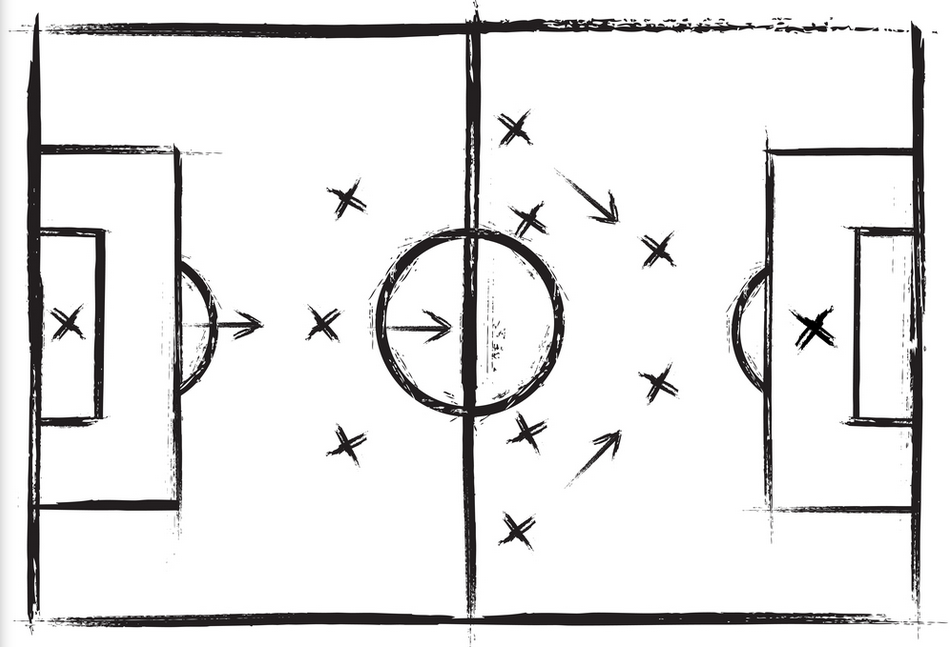
\includegraphics[width=0.27\textwidth]{img/trener.png}
\end{wrapfigure}

Do sada smo već shvatili da studenti vole spavati. Patrik je apsolutni rekorder
u toj kategoriji. Probudi se jedino ako mora nešto pojesti ili ako želi
igrati igru \textit{FIFA 20}. Zbog previše igranja, njegovi su snovi nerijetko
povezani s nogometom. U posljednjem snu našao se u ulozi, ni manje ni više,
nego trenera GNK Dinamo Zagreb, inače njegovog najdražeg nogometnog kluba.

Njegov posao je odabrati $N$ igrača koji će u sljedećoj sezoni igrati u modrim
dresovima, no uprava kluba ima čudne zahtjeve za odabir igrača. Zahtjevi su:

\begin{itemize}
  \item svi igrači moraju imati različit broj slova u prezimenu.
  \item prezime igrača se mora nalaziti kao uzastopni podniz u prezimenima svih
        igrača čija prezimena imaju više slova.
\end{itemize}

Kako bi si olakšao posao, Patrik je podijelio igrače u $N$ skupina na način da
igrači u skupini $i$ imaju točno $i$ slova u prezimenu. U svakoj od tih
skupina nalazi se točno $K$ igrača. Patrika zanima na koliko različitih
načina (modulo $10^9 + 7$) može odabrati igrače za svoju momčad, a da uvjeti
uprave kluba budu ispunjeni.

%%%%%%%%%%%%%%%%%%%%%%%%%%%%%%%%%%%%%%%%%%%%%%%%%%%%%%%%%%%%%%%%%%%%%%
% Input
\subsection*{Ulazni podaci}
U prvom su retku prirodni brojevi $N$ $(1 \le N \le 50)$ i $K$ $(1 \le K \le 1\
500)$

U svakom od sljedećih $N$ redaka je $K$ ne nužno različitih prezimena igrača
odvojenih razmakom. Prezimena igrača u $i$-tom retku imaju točno $i$ malih slova
engleske abecede.

%%%%%%%%%%%%%%%%%%%%%%%%%%%%%%%%%%%%%%%%%%%%%%%%%%%%%%%%%%%%%%%%%%%%%%
% Output
\subsection*{Izlazni podaci}
U jedini redak ispišite traženi broj iz teksta zadatka.

%%%%%%%%%%%%%%%%%%%%%%%%%%%%%%%%%%%%%%%%%%%%%%%%%%%%%%%%%%%%%%%%%%%%%%
% Scoring
\subsection*{Bodovanje}
{\renewcommand{\arraystretch}{1.4}
  \setlength{\tabcolsep}{6pt}
  \begin{tabular}{ccl}
 Podzadatak & Broj bodova & Ograničenja \\ \midrule
  1 & 22 & $N = 5$ i $K = 10$ \\
  2 & 33 & $N = 50$ i $K = 100$\\
  3 & 30 & Nema dodatnih ograničenja. \\
\end{tabular}}

%%%%%%%%%%%%%%%%%%%%%%%%%%%%%%%%%%%%%%%%%%%%%%%%%%%%%%%%%%%%%%%%%%%%%%
% Examples
\subsection*{Probni primjeri}
\begin{tabularx}{\textwidth}{X'X'X}
\sampleinputs{test/trener.dummy.in.1}{test/trener.dummy.out.1} &
\sampleinputs{test/trener.dummy.in.2}{test/trener.dummy.out.2} &
\sampleinputs{test/trener.dummy.in.3}{test/trener.dummy.out.3}
\end{tabularx}

\textbf{Pojašnjenje prvog probnog primjera:}
Patrik može odabrati sljedeće ekipe: \texttt{(a, ab, abc)}, \texttt{(a, ab, abd)},
\texttt{(b, ab, abc)}, \texttt{(b, ab, abd)} i \texttt{(b, bd, abd)}.

%%%%%%%%%%%%%%%%%%%%%%%%%%%%%%%%%%%%%%%%%%%%%%%%%%%%%%%%%%%%%%%%%%%%%%
% We're done
\end{statement}

%%% Local Variables:
%%% mode: latex
%%% mode: flyspell
%%% ispell-local-dictionary: "croatian"
%%% TeX-master: "../hio.tex"
%%% End:
